\documentclass[tikz]{standalone}
\usetikzlibrary{automata,positioning}
\begin{document}
	
	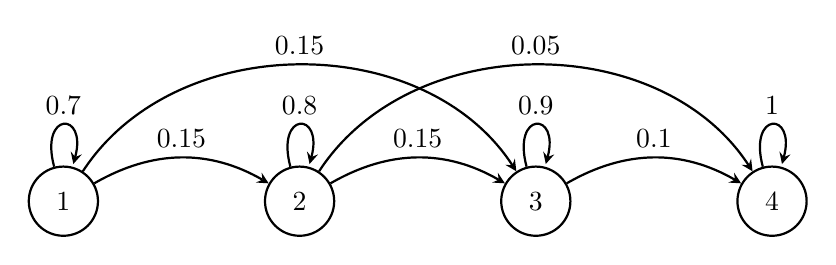
\begin{tikzpicture}[>=stealth,node distance=3cm,on grid,auto, thick, initial text=] 
		\node[state]         (P_1)   {$1$}; 
		\node[state]         (P_2)   [right=3cm of P_1] {$2$};
		\node[state]         (P_3)   [right=3cm of P_2] {$3$};
		\node[state]         (P_4)   [right=3cm of P_3] {$4$};
		
		\path[->]            (P_1) edge [bend left] node [above] {0.15} (P_2)
		edge [bend left=2cm] node [above] {0.15} (P_3)
		(P_2) edge [bend left] node[above] {0.15} (P_3)
		edge [bend left=2cm] node[above] {0.05} (P_4)
		(P_3) edge [bend left] node[above] {0.1} (P_4)
		
		(P_1) edge [loop above] node {0.7} (P_1)
		(P_2) edge [loop above] node {0.8} (P_2)
		(P_3) edge [loop above] node {0.9} (P_3)
		(P_4) edge [loop above] node {1} (P_4);
	\end{tikzpicture}
\end{document}
